\newcommand{\difference}[1]{\mathrm{\Delta} #1}

\section{Einleitung}

Das LHCb-Experiment beschäftigt sich zur Überprüfung des Standardmodells der Teilchenphysik mit Präzisionsmessungen an Zerfällen von \PB-Mesonen.

Eine der am LHCb-Detektor durchgeführten Messungen ist die Bestimmung der zeitabhängigen \textit{CP}-Verletzung in den Zerfällen neutraler \PB-Mesonen.
Wichtig ist dabei die Bestimmung der Produktionszustände der erzeugten \PB-Mesonen, die als Flavour-Tagging bezeichnet wird.
In diesem Zusammenhang muss die Fehlerrate der Tagging-Entscheidungen, auch Mistag-Wahrscheinlichkeit genannt, möglichst genau bekannt sein.

Diese Bachelorarbeit beschäftigt sich mit der Flavour-Tagging-Kalibration, die das Ziel hat, eine möglichst genaue Abschätzung der Mistag-Wahrscheinlichkeit zu liefern.
Sie basiert auf einem Datensatz rekonstruierter $\PBz \to \PJpsi\,\PKst^0$-Zerfälle, der im Jahr 2012 aufgenommen wurde und konzentriert sich auf eine Kalibration des Same-Side-Pion-Taggers (SS\Pgp).
In früheren Analysen \cite{sin2beta} hat sich gezeigt, dass dieser einen Zugewinn von ca. \SI{25}{\percent} in der statistischen Sensitivität gegenüber der Kombination aller anderen Tagger für die Analyse zeitabhängiger \textit{CP}-Verletzung in \PBz-Zerfällen ausmacht.
Im Gegensatz zu anderen Taggern liefert eine Kalibration des SS\Pgp mittels Zerfällen geladener \PB-Mesonen nur ungenügende Ergebnisse, weshalb er durch Zerfälle neutraler \PB-Mesonen in flavour-spezifische Endzustände kalibriert werden muss.

Im Folgenden gilt die Konvention $\hbar = c = 1$.

\newpage

\section{Standardmodell der Teilchenphysik}
\label{standard-model}

Das Standardmodell der Teilchenphysik ist eine Quantenfeldtheorie, die alle bislang bekannten Elementarteilchen und ihre Interaktionen über die starke, schwache und elektromagnetische Wechselwirkung beschreibt.

Die Elementarteilchen lassen sich in Quarks und Leptonen, aus denen Materie besteht, und Eichbosonen, die Kräfte zwischen den Teilchen vermitteln, unterteilen.
Das Standardmodell ist ausgesprochen erfolgreich: Seine Vorhersagen decken sich mit jedem bisher durchgeführten Experiment der Hochenergiephysik.

Dennoch kann es sich dabei nicht um eine vollständige Theorie aller physikalischen Effekte handeln.
So gibt es noch keine allgemein akzeptierte Methode, um die Gravitation in das Standardmodell einzubeziehen.
Außerdem ist eine Reihe von Phänomenen bekannt, die sich nicht durch das Standardmodell erklären lassen, wie das Vorhandensein und die Natur von dunkler Materie und dunkler Energie, die Größe der beobachteten Materie-Antimaterie-Asymmetrie im Universum, sowie die Existenz der Neutrinomassen.

Eine Möglichkeit Anzeichen für sogenannte ,,Neue Physik'' zu finden, ist es mittels hochpräziser Experimente, wie sie z.B. am LHCb-Detektor stattfinden, nach Abweichungen von den Vorhersagen des Standardmodells zu suchen.

\subsection{Quark-Sektor im Standardmodell}

Das Standardmodell beinhaltet sechs verschiedene Arten von Quarks: up, down, charm, strange, top und bottom.
Diese werden als \Pqu, \Pqd, \Pqc, \Pqs, \Pqt und \Pqb abgekürzt und in drei Familien unterteilt:
\begin{eqn}
  \begin{pmatrix}
    \Pqu & \Pqc & \Pqt \\
    \Pqd & \Pqs & \Pqb \\
  \end{pmatrix}
  \eqlabel{quarks}
\end{eqn}
Alle sechs sogenannten Quark-Flavour besitzen unterschiedliche Massen.

Ein erster experimenteller Beleg für die Existenz von Quarks wurde 1969 am Stanford Linear Accelerator (SLAC) durch Elektron-Streuexperimente (Deep Inelastic Scattering) an Protonen demonstriert \cite{slac-quarks}.

Quarks besitzen eine elektrische Ladung, wechselwirken also elektromagnetisch.
Up-type Quarks (die obere Zeile in \eqref{quarks}) besitzen eine Ladung von $+⅔$, down-type Quarks (die untere Zeile) eine Ladung von $-⅓$.
Zu jedem der Quarks existiert ein Antiquark mit gleicher Masse und umgekehrter Ladung.

Quarks sind die einzigen bekannten Elementarteilchen, die an die Austauschteilchen der starken Wechselwirkung, die Gluonen, koppeln.
Jedes Quark besitzt dazu eine sogenannte Farbladung.
Beobachtet werden können nur gebundene Quark-Zustände, deren Farbladungen sich zu Null addieren.
Diese bezeichnet man als Hadronen.

Quarks wechselwirken zusätzlich über die schwache Wechselwirkung.
Im Gegensatz zur elektromagnetischen und starken Wechselwirkung erhält diese nicht den Quark-Flavour, da die Eigenzustände der schwachen Wechselwirkung ungleich den Flavour-Eigenzuständen sind.
So kann ein Quark unter Abgabe eines \PW-Bosons von einem up-type Quark zu einem down-type Quark und umgekehrt werden.
Es finden dabei auch Wechsel zwischen den Quark-Familien statt, diese treten aber mit einer geringeren Wahrscheinlichkeit als Wechsel innerhalb einer Familie auf.
Die Eigenzustände lassen sich über die unitäre Cabibbo-Kobayashi-Maskawa-Matrix (CKM-Matrix) über
\begin{eqn}
  \begin{pmatrix}
    \Pqd' \\
    \Pqs' \\
    \Pqb' \\
  \end{pmatrix}
  =
  \begin{pmatrix}
    V_{\Pqu\Pqd} & V_{\Pqu\Pqs} & V_{\Pqu\Pqb} \\
    V_{\Pqc\Pqd} & V_{\Pqc\Pqs} & V_{\Pqc\Pqb} \\
    V_{\Pqt\Pqd} & V_{\Pqt\Pqs} & V_{\Pqt\Pqb} \\
  \end{pmatrix}
  \begin{pmatrix}
    \Pqd \\
    \Pqs \\
    \Pqb \\
  \end{pmatrix}
\end{eqn}
ineinander umwandeln.
Sie übersetzt die Flavour-Eigenzustände 
\begin{eqn}
  \begin{pmatrix}
    \Pqu \\  
    \Pqd \\  
  \end{pmatrix}
  ,
  \begin{pmatrix}
    \Pqc \\ 
    \Pqs \\ 
  \end{pmatrix}
  ,
  \begin{pmatrix}
    \Pqt \\ 
    \Pqb \\ 
  \end{pmatrix}
\end{eqn}
in Eigenzustände der schwachen Wechselwirkung
\begin{eqn}
  \begin{pmatrix}
    \Pqu\phantom{'} \\  
    \Pqd' \\  
  \end{pmatrix}
  ,
  \begin{pmatrix}
    \Pqc\phantom{'} \\ 
    \Pqs' \\ 
  \end{pmatrix}
  ,
  \begin{pmatrix}
    \Pqt\phantom{'} \\ 
    \Pqb' \\
  \end{pmatrix}\:.
\end{eqn}
Die Betragsquadrate ihrer Einträge geben die Wahrscheinlichkeiten für einen Flavour-Wechsel an.

Im Folgenden soll auf den Begriff der $CP$-Verletzung näher eingegangen werden.

\subsection{CP-Verletzung im Standardmodell}

\newcommand{\Vud}{V_{\Pqu\Pqs}}
\newcommand{\Vus}{V_{\Pqu\Pqs}}
\newcommand{\Vub}{V_{\Pqu\Pqb}}
\newcommand{\Vcd}{V_{\Pqc\Pqd}}
\newcommand{\Vcs}{V_{\Pqc\Pqs}}
\newcommand{\Vcb}{V_{\Pqc\Pqb}}
\newcommand{\Vtd}{V_{\Pqt\Pqd}}
\newcommand{\Vts}{V_{\Pqt\Pqs}}
\newcommand{\Vtb}{V_{\Pqt\Pqb}}

Drei diskrete Symmetrieoperatoren sind im Standardmodell von Interesse:
die Ladungskonjugation $C$, die die ladungsartigen Quantenzahlen aller Teilchen im System umkehrt,
die Parität $P$, die das System im Ursprung spiegelt und
die Zeitumkehr $T$, die den Zeitfluss des Systems umkehrt.

Lange Zeit dachte man, dass die Physik unter Anwendung von $P$ invariant bliebe.
Ein 1956 von Lee und Yang postuliertes \cite{cp-lee-yang} und von Wu durchgeführtes \cite{wu} Experiment zeigte aber, dass dies nicht der Fall ist.

Daraufhin nahm man an, dass die Kombination aus Ladungskonjugation und Paritätsumkehr, $CP$, eine universelle Symmetrie darstellen würde.
Doch auch das konnte im neutralen Kaon-System von Cronin, Fitch, u.a 1964 widerlegt werden \cite{kaons-cronin-fitch}.

$CP$-Verletzung wurde ausschließlich in hadronischen Systemen beobachtet.
Sie ist im Standardmodell als komplexe Phase in der CKM-Matrix verwirklicht.
Die Tatsache, dass dieser Mechanismus nur bei Existenz von mindestens drei Quarkfamilien funktioniert, inspirierte Kobayashi und Maskawa 1973 dazu, die Existenz der damals noch nicht entdeckten dritten Quarkfamilie (mit Top-Quark und Bottom-Quark) zu postulieren \cite{kobayashi-maskawa}.
Dafür erhielten beide 2008 den Nobelpreis.

Ist die CKM-Matrix unitär, so verschwinden jeweils die komplexen Skalarprodukte zweier verschiedener Spalten.
Die Produkte bestehen jeweils aus drei komplexen Termen.
Zum Beispiel gilt für das Produkt der ersten und der dritten Spalte
\begin{eqn}
  \Vud^{}\Vub^* + \Vcd^{}\Vcb^* + \Vtd^{}\Vtb^* = 0\:.
\end{eqn}
Die drei Terme können als Linien in der komplexen Ebene visualisiert werden, die sich zu einem Dreieck schließen.
Nützlich ist es, jede der Seiten auf $\Vcd\Vcb^*$ zu normieren; die einzigen freien Parameter sind dann die Koordinaten $\bar{ρ}$ und $\bar{η}$ der Dreiecks-Spitze (siehe Abb. \ref{unitarity-triangle}).
Der Flächeninhalt der Dreiecke ist dabei ein Maß für den Grad der \textit{CP}-Verletzung.

\begin{figure}
  \centering
  \begin{tikzpicture}[scale=6]
    \coordinate (A) at (0.225,0.345);
    \coordinate (B) at (1,0);
    \coordinate (C) at (0,0);

    \node [above] at (0.225,0.365) {$(\bar{ρ},\bar{η})$};
    \node [below] at (0, -0.02) {$(0,0)$};
    \node [below] at (1, -0.02) {$(1,0)$};

    \draw (A) -- node[above right] {$\abs{\frac{\Vtd \Vtb^*}{\Vcd \Vcb^*}}$} (B) -- node[below] {$1$} (C) -- node[above left] {$\abs{\frac{\Vud \Vub^*}{\Vcd \Vcb^*}}$} (A);

    \begin{scope}
      \path[clip] (A) -- (B) -- (C) -- cycle;
      \draw (A) circle (0.17);
      \draw (B) circle (0.3);
      \draw (C) circle (0.19);
    \end{scope}

    \node at (0.240,0.260) {$α$};
    \node at (0.77,0.045) {$β$};
    \node at (0.10,0.06) {$γ$};

  \end{tikzpicture}
  \caption{Das Unitaritätsdreieck $\Vud\Vub^* + \Vcd\Vcb^* + \Vtd\Vtb^* = 0$ mit Seitenlängen normiert auf $\Vcd\Vcb^*$.
  Das transformierte Dreieck ist vollständig durch die Lage der Dreiecks-Spitze festgelegt.
  Dieses Dreieck wird oft als \enquote{das} Unitaritätsdreieck bezeichnet, da es im Vergleich zu den anderen möglichen Dreiecken am wenigsten entartet ist.}
  \label{unitarity-triangle}
\end{figure}

Interessant ist, dass die somit vom Standardmodell vorhergesagte \textit{CP}-Verletzung sich mit jedem bisherigen Experiment gedeckt hat, obwohl die vorhergesagte Größe nicht dazu in der Lage ist, die im Universum beobachtete Ma\-te\-rie-Anti\-materie-Asymmetrie zu erklären.

Eine Möglichkeit, den CKM-Mechanismus auf seine Gültigkeit zu überprüfen, ist experimentell die Lage der Dreiecks-Spitze aus Abb. \ref{unitarity-triangle} einzuschränken, sie sogar regelrecht überzubestimmen.
Widersprüche oder Abweichungen von der Theorie würden dann z.B. darauf hindeuten, dass es weitere Elementarteilchen geben könnte, die im Standardmodell nicht beachtet wurden.

In diesem Zusammenhang wurden zahlreiche Experimente durchgeführt.
Ein äußerst aussagekräftiges Experiment, welches bei LHCb durchgeführt wird, ermöglicht die Bestimmung des Winkels $β$ und basiert auf der Oszillation neutraler \PB-Mesonen. Das Experiment wurde bereits von den BaBar- und Belle-Kollaborationen durchgeführt \cite{babar-sin2beta}\cite{belle-sin2beta}.

\subsection{$\PB$-$\PaB$-Oszillation}

Als \PB-\PaB-Oszillation bezeichnet man die Tatsache, dass neutrale \PB-Mesonen bei freier Propagation je nach Lebensdauer eine bestimmte Wahrscheinlichkeit haben, als ihr Antiteilchen zu zerfallen.
Die Oszillation neutraler Mesonen war bereits von Cronin und Fitch im Kaon-System verwendet worden, um \textit{CP}-Verletzung zu demonstrieren \cite{kaons-cronin-fitch}.
Dass auch neutrale \PB-Mesonen eine Oszillation aufweisen, wurde 1987 von der Argus-Kollaboration am DESY gezeigt \cite{argus-bbar}.

Anhand der beiden Feynman-Diagramme in Abb. \ref{bbar-oscillation} lässt sich verstehen, dass Amplituden für die Übergänge eines $\PBz$ zu seinem Antiteilchen und umgekehrt existieren.

\begin{figure}
  \begin{tikzpicture}[line width=1.2 pt, scale=1.1]
    \draw[fermion] (-1,2.3) node [left] {\Pqd} -- (0,2);
    \draw[fermion] (0,2) -- node [above] {$\Pqu,\Pqc,\Pqt$} (2, 2);
    \draw[fermion] (2,2) -- (3,2.3) node [right] {\Pqb};
     
    \draw[fermionbar] (-1,-.3) node [left] {\Paqb} -- (0,0);
    \draw[fermionbar] (0,0) -- node [above] {$\Pqu,\Pqc,\Pqt$} (2,0);
    \draw[fermionbar] (2,0) -- (3,-.3) node [right] {\Paqd};
    
    \draw[vector] (0,2) -- node [left] {\PW} (0,0);
    \draw[vector] (2,2) -- node [right] {\PW} (2,0);
  \end{tikzpicture}
  \hspace{1cm}
  \begin{tikzpicture}[line width=1.2 pt, scale=1.1]
    \draw[fermion] (-1,2.3) node [left] {\Pqd} -- (0,2);
    \draw[vector] (0,2) -- node [above] {\PWm} (2, 2);
    \draw[fermion] (2,2) -- (3,2.3) node [right] {$b$};
     
    \draw[fermionbar] (-1,-.3) node [left] {\Paqb} -- (0,0);
    \draw[vector] (0,0) -- node [above] {\PWp} (2,0);
    \draw[fermionbar] (2,0) -- (3,-.3) node [right] {\Paqd};
    
    \draw[fermion] (0,2) -- node [left] {$\Pqu,\Pqc,\Pqt$} (0,0);
    \draw[fermionbar] (2,2) -- node [right] {$\Pqu,\Pqc,\Pqt$} (2,0);
  \end{tikzpicture}
  \caption{Feynman-Diagramme der \PBz-\PaBz-Oszillation.
  In dieser Ordnung ergibt sich die Amplitude für einen Flavour-Wechsel als Summe beider Diagramme.}
  \label{bbar-oscillation}
\end{figure}

Im Folgenden sollen die Übergangswahrscheinlichkeiten für $\PBz \to \PBz$ und $\PBz \to \PaBz$ bestimmt und damit eine Wahrscheinlichkeitsdichte für die Messung gemischter und ungemischter Zerfälle ermittelt werden.

Die Herleitung orientiert sich an \cite{babar-book} und \cite{spaan}.

Zu jedem Zeitpunkt lässt sich der Zustand des \PBz-\PaBz-Systems in der Breit-Wigner-Näherung als Superposition
\begin{eqn}
  ψ = a \ket{\PBz} + b \ket{\PaBz}
\end{eqn}
schreiben.
Der zugehörige Hamiltonian, der Zerfall und Übergang der beiden Zustände beschreibt, ist durch
\begin{eqn}
  \renewcommand*{\arraystretch}{1.5}
  H = 
  \begin{pmatrix}
    M_{11}-\frac{\I}{2} Γ_{11} & M_{12}-\frac{\I}{2} Γ_{12} \\
    M^*_{12}-\frac{\I}{2} Γ^*_{12} & M_{22}-\frac{\I}{2} Γ_{22} \\
  \end{pmatrix}
\end{eqn}
gegeben.
Durch Diagonalisierung von $H$ erhält man die Masseneigenzustände
\begin{eqns}
  \ket{\PB_\t{L}} &=& p \ket{\PBz} + q \ket{\PaBz} \\
  \ket{\PB_\t{H}} &=& p \ket{\PBz} - q \ket{\PaBz}
\end{eqns}
mit
\begin{eqn}
  \frac{q}{p} = \frac{\difference{m_{\Pqd}} - \frac{\I}{2}\difference{Γ_{\Pqd}}}{2M_{12} - \frac{\I}{2}\difference{Γ_{\Pqd}}}\:.
\end{eqn}
Dabei ist $\difference{m_{\Pqd}}$ der Unterschied $M_\t{H} - M_\t{L}$ zwischen den Massen der beiden Eigenzustände und gibt die Frequenz der \PBz-\PaBz-Oszillation an, während $\difference{Γ_{\Pqd}}$ die Differenz ihrer Zerfallsbreiten angibt, welche im \PBz-System nahezu verschwindet.

Die Zeitentwicklung der beiden Zustände lautet dann
\begin{eqns}
  \ket{\PBz(t)} &=& g_+(t) \ket{\PBz} + \frac{q}{p} g_-(t)\ket{\PaBz} \\
  \ket{\PaBz(t)} &=& \frac{p}{q} g_-(t) \ket{\PBz} + g_+(t)\ket{\PaBz}
\end{eqns}
mit
\begin{eqns}
  g_+(t) &=& \E^{-\I M t} \E^{-½Γt} \cos(Δm_{\Pqd} t/2) \\
  g_-(t) &=& \E^{-\I M t} \E^{-½Γt} \I\sin(Δm_{\Pqd} t/2)\:,
\end{eqns}
wobei $M=\frac{M_L + M_H}{2}$ und $Γ=\frac{Γ_L + Γ_H}{2}$ gilt.

Im Folgenden soll die Näherung $\frac{p}{q} = 1$ gemacht werden, was bedeutet, dass die Asymmetrie zwischen den Übergängen $\PBz\to\PaBz$ und $\PaBz\to\PBz$ (indirekte \textit{CP}-Verletzung) vernachlässigt wird.

Für die Wahrscheinlichkeiten, dass ein Meson nach einer Zeit $t$ seinen Flavour behalten ($q=+1$) oder geändert ($q=-1$) hat, gilt dann
\begin{eqn}
  \braket{\PBz(t)}{\PBz(0)}^2 = \braket{\PaBz(t)}{\PaBz(0)}^2 = \frac{1}{4} (\E^{-Γ_L t} + \E^{-Γ_H t} + 2\E^{\frac{-Γ}{2}t}) \cos(\difference{m_{\Pqd}}t)
\end{eqn}
\begin{eqn}
  \braket{\PaBz(t)}{\PBz(0)}^2 = \braket{\PBz(t)}{\PaBz(0)}^2 = \frac{1}{4} (\E^{-Γ_L t} + \E^{-Γ_H t} - 2\E^{\frac{Γ}{2}t}) \cos(\difference{m_{\Pqd}}t)\:.
\end{eqn}

Da die beiden Massen-Eigenzustände im \PB-System annähernd identische Zerfallsbreiten aufweisen, lässt sich die Formel mittels $Γ_L = Γ_H = Γ$ zu
\begin{eqn}
  P_{q=\pm1}(t) = \frac{1}{2} \exp(-Γt) \g(1 \pm \cos(\difference{m_{\Pqd}}t))
  \eqlabel{mixing-probability}
\end{eqn}
nähern.
Diese Formel wird in der Analyse in modifizierter Form für einen Fit der gemessenen \PB-Zerfälle verwendet.

Angenommen man kennt die Produktions- und Endzustände gemessener \PB-Zerfälle, dann gilt für die Anzahl der ermittelten gemischten und ungemischten Zerfallsereignisse mit Zerfallszeit $t$
\begin{eqn}
  N_{q=\pm1}(t) = N_\t{sig} P_{q=\pm1}(t)\:.
\end{eqn}

Die Asymmetrie der gemessenen Signalereignisse mit und ohne Mixing lässt sich damit über
\begin{eqn}
  M_\t{sig}(t) = \frac{N_{q=+1}(t) - N_{q=-1}(t)}{N_{q=+1}(t) + N_{q=-1}(t)} = \cos(\difference{m_{\Pqd}} t)
  \eqlabel{mixing}
\end{eqn}
bestimmen.

% B⁰ → J/ψ K*
%\begin{tikzpicture}[line width=1.2 pt, scale=2]
%  \draw[fermion] (0, 0.5) node [left] {\Pqd} -- (2, 0.5) node [right] {\Pqd};
%  \draw[fermionbar] (0, 0) node [left] {\Pqb} -- (0.75, 0);
%  \draw[fermionbar] (1.25, 0) -- (2, 0) node [right] {\Pqs};
%  \draw[vector] (0.75, 0) -- node [above] {\PW} (1.25, 0);
%  \draw[fermion] (1.25, 0) -- (2, -0.5) node [below] {\Pqc};
%  \draw[fermionbar] (0.75, 0) -- (1.500, -0.5) node [below] {\Pqc};
%\end{tikzpicture}

\section{Experimentelle Grundlagen}

\subsection{Der LHCb-Detektor}

Der Large Hadron Collider beauty Detektor (LHCb) ist Grundlage eines der vier größten Experimente, die am Large Hadron Collider (LHC) nahe Genf durchgeführt werden.

Er wurde vorrangig gebaut, um Zerfälle von \PB-Mesonen auf indirekte Anzeichen für Neue Physik zu untersuchen.

Im Gegensatz zu den anderen großen Detektoren am LHC (ATLAS, CMS und ALICE) handelt es sich hierbei nicht um einen $4\PI$-Detektor, sondern um ein einarmiges Vorwärtsspektrometer mit einer Winkelakzeptanz von \SIrange{10}{300}{\radian}. Dies ist angesichts der Tatsache, dass bereits ca. ¼ der \PB-\PaB-Paare in diesem Winkelbereich erfasst werden können, sinnvoll.

Er ist für eine vergleichsweise geringe Luminosität, gleichzeitig aber für eine hochpräzise Rekonstruktion ausgelegt.

Die folgenden Informationen sind aus \cite{lhcb} entnommen.
Ein Querschnitt des Detektors ist in Abbildung \ref{lhcb} dargestellt.

Der Vertex Locator (VELO) ist ein Siliziumdetektor, der aus zwei Hälften besteht und bis auf \SI{5}{\milli\metre} an den Protonenstrahl herangefahren werden kann. Er wird zur Vertex-Rekonstruktion und zur Messung von Stoßparametern verwendet. Er ist in der Lage, Entfernungen von \SI{10}{\micro\metre} aufzulösen.
Das entspricht einer Eigenzeitauflösung von ca. \SI{50}{\femto\second} für \PB-Mesonen.

Die beiden Ring Imaging Cherenkov (RICH) Detektoren messen mittels Cherenkov-Strahlung die Geschwindigkeit geladener Teilchen, was durch Vergleich mit Informationen aus dem Tracking eine Bestimmung der Teilchenmassen erlaubt und damit zusammen mit der Information über Ladung und Impuls des Teilchens seine Identifizierung (PID) ermöglicht.

Der konventionelle (nicht supraleitende) Dipolmagnet verfügt über ein integriertes Magnetfeld von \SI{4}{\tesla\meter}.

Die Trackerstationen T1 bis T3 ermöglichen eine Verfolgung der Teilchenbahnen.

Dahinter befinden sich die elektromagnetischen und hadronischen Kalorimeter, die Elektronen, Photonen und Hadronen auf"|fangen und ihre Energie messen.

Am Ende des Detektors befindet sich eine Reihe von Drahtkammern (M2 bis M5), die eine Identifikation von Myonen ermöglichen.
Zwischen den Drahtkammern sind Bleiplatten als sogenannte Myon-Filter angebracht.
Diese lassen Myonen passieren, während Hintergrundstrahlung nach dem Durchtritt mehrerer Platten gestoppt wird und somit als Myon-Ereignis ausgeschlossen werden kann.

\begin{figure}
  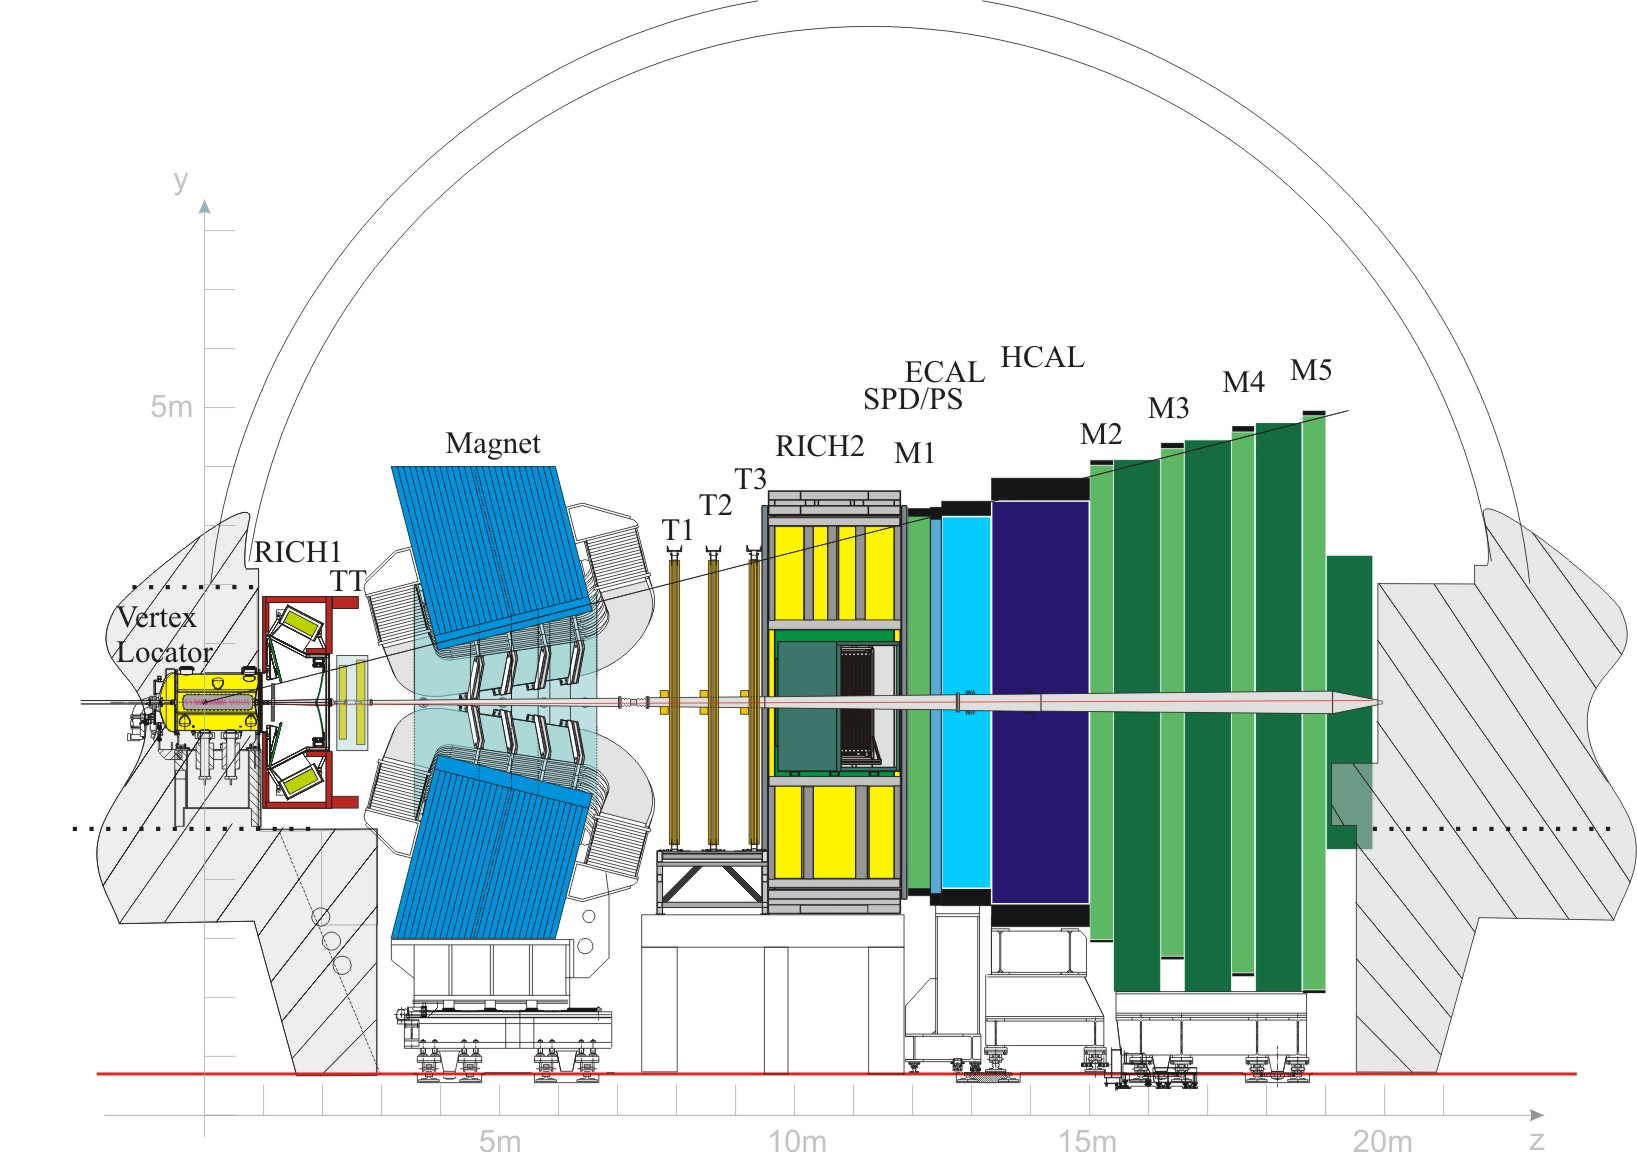
\includegraphics[width=\textwidth]{figures/lhcb.pdf}
  \caption{Querschnitt des LHCb-Detektors. Die einzelnen Komponenten werden im Text erläutert \cite{lhcb}.}
  \label{lhcb}
\end{figure}

\subsection{Flavour-Tagging}

Zur Bestimmung der Oszillations\-frequenz $\difference{m_{\Pqd}}$ der produzierten $\PBz$- und $\PaBz$-Mesonen muss neben den Zerfallszeiten der einzelnen beobachteten Mesonen sowohl deren End- als auch deren Anfangszustand bekannt sein.

Der Endzustand kann aus den Zerfallsprodukten der \PBz und \PaBz Mesonen bestimmt werden, wenn man einen Kanal mit selbst-taggendem Endzustand wählt.
Zu diesen Kanälen gehören $\PBz \to \PJpsi\,\PKst^0$ in guter Näherung $\PBz \to \PDm \Pgpp$.
Im Fall von $\PBz\to\PJpsi\,\PKst^0$ zerfällt das $\PKst^0$ in $\PKp\Pgpm$, sodass eine Identifikation des Endzustandes über die Kaon-Ladung möglich ist.

Die Bestimmung des Anfangszustandes (\PBz oder \PaBz), die man als Flavour-Tagging bezeichnet, erweist sich als deutlich schwieriger.
Das LHCb-Experiment verwendet hierzu neuronale Netze (genauer: Multilayer Perceptrons), welche darauf trainiert werden, aus der Beobachtung gleichzeitig mit dem \PBz entstandener, geladener Mesonen Rückschlüsse auf den Flavour des \PBz-Mesons zu ziehen.
Diese sogenannten Tagger lassen sich in zwei Typen unterteilen: Opposite-Side-Tagger (OST) und Same-Side-Tagger (SST).
Außerdem gibt es noch den Vertex-Charge-Tagger, auf den hier aber nicht näher eingegangen werden soll.

\begin{figure}
  \centering
  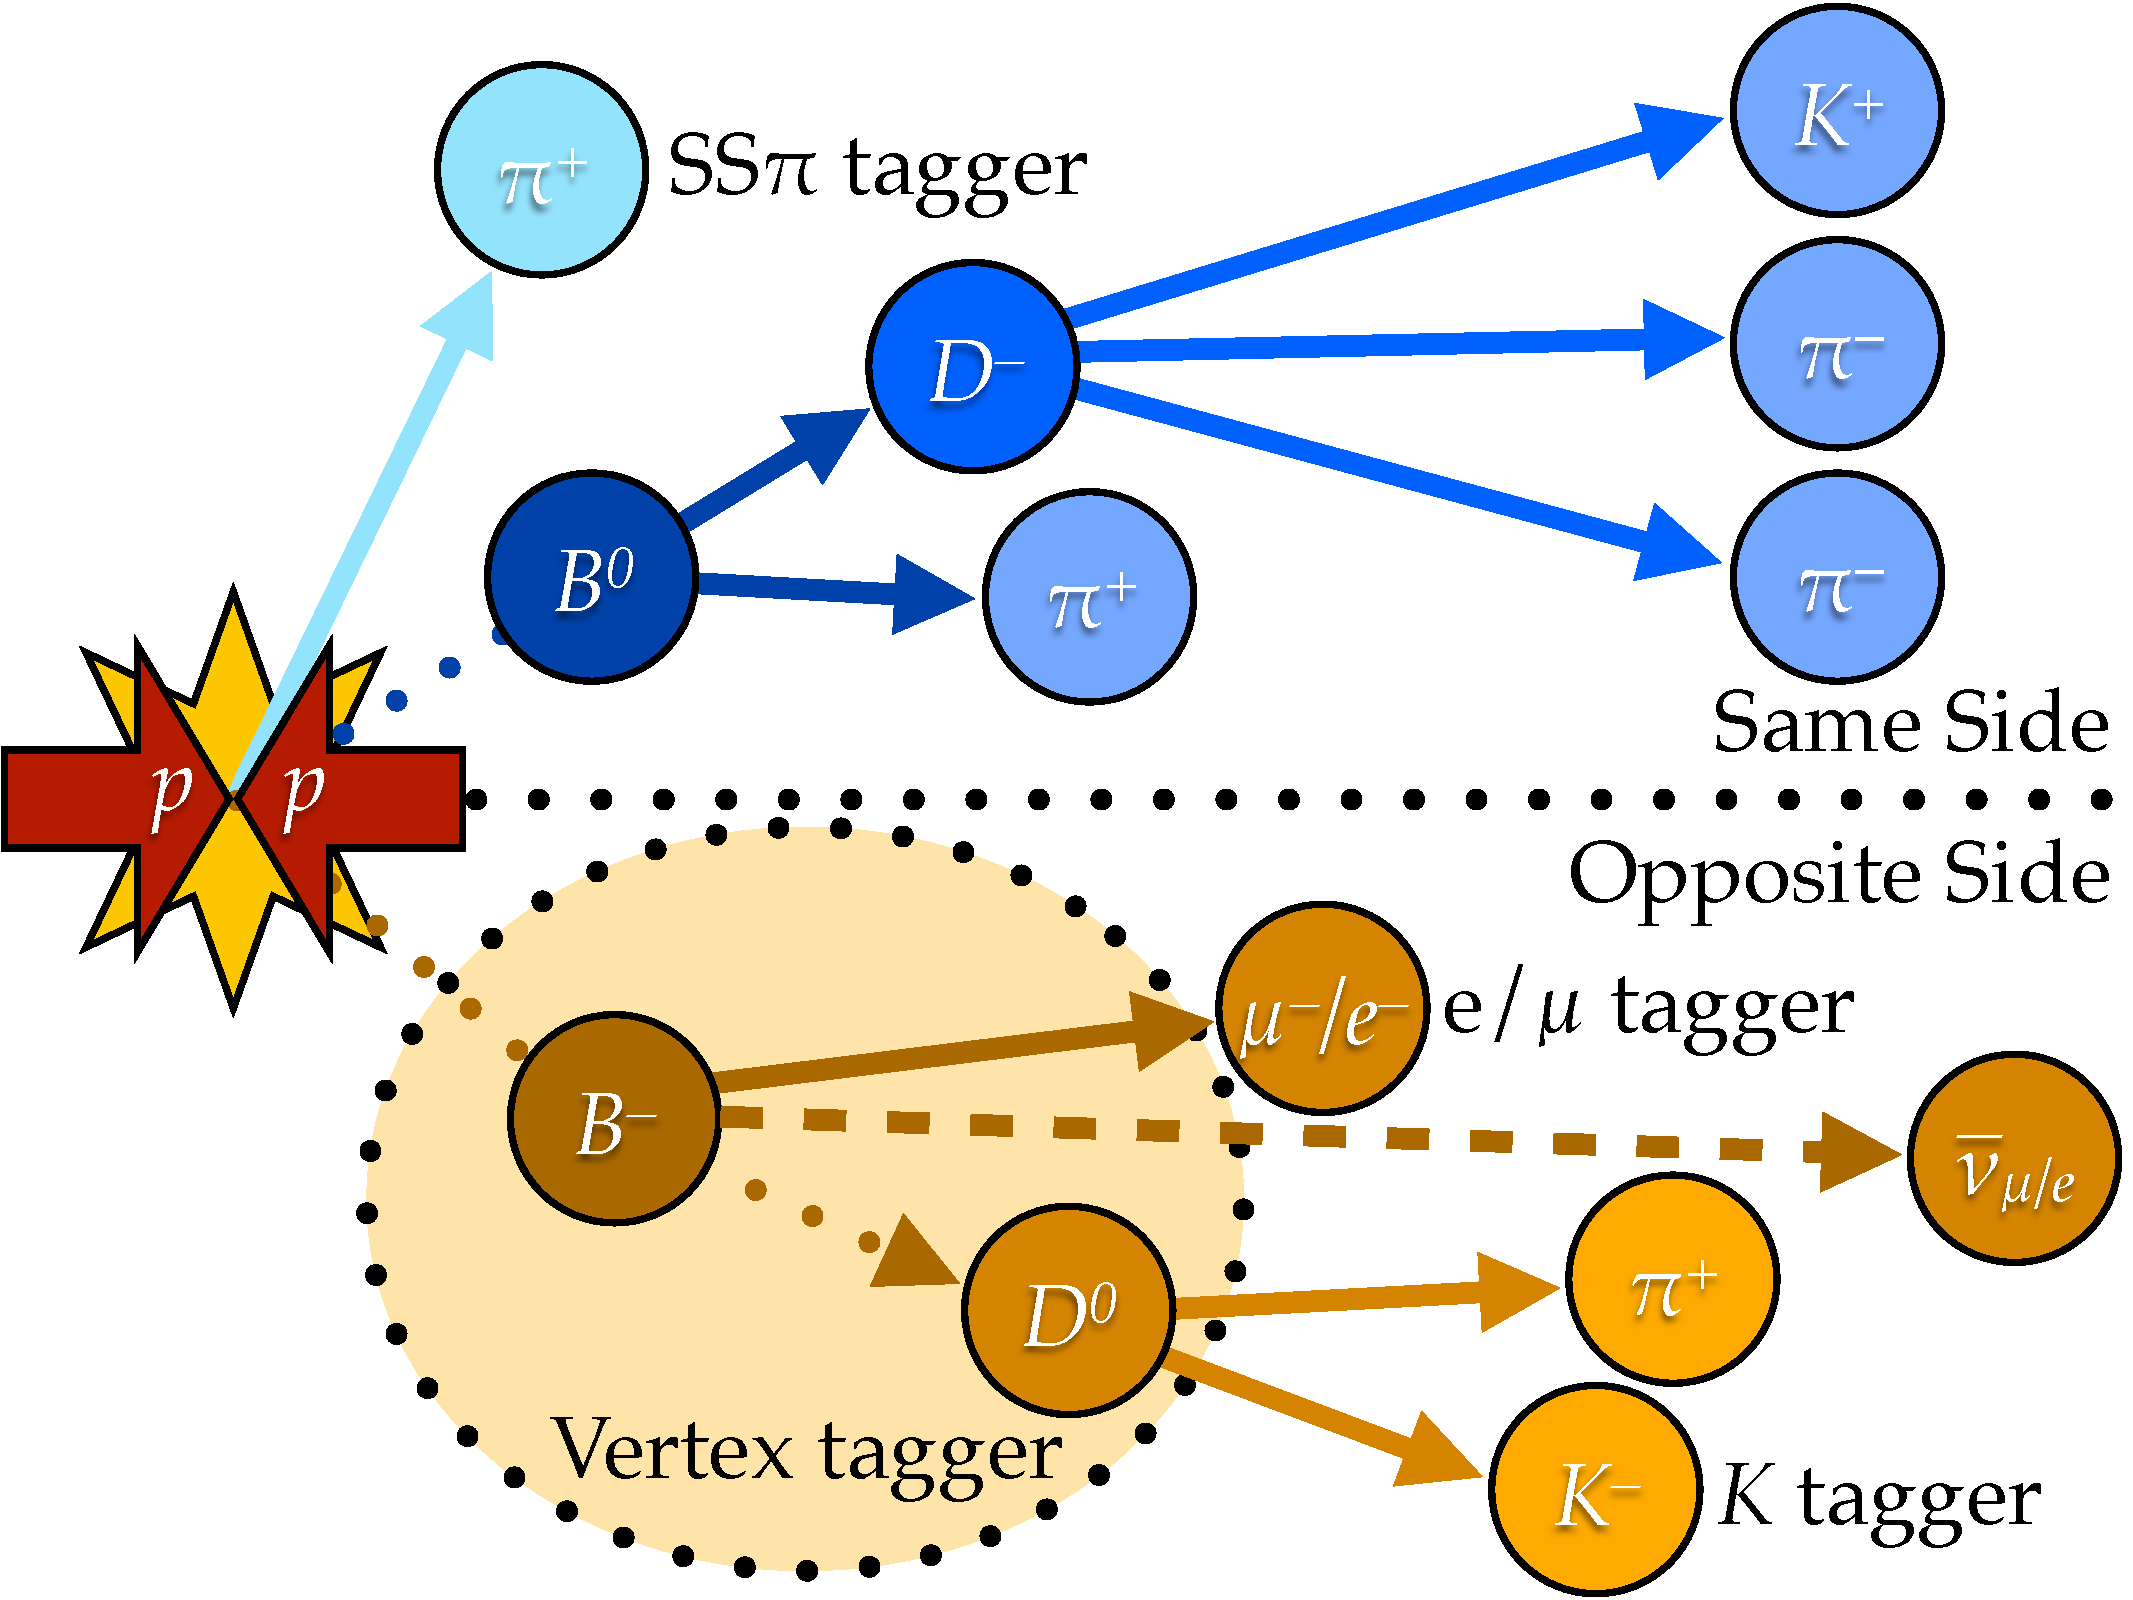
\includegraphics[width=0.6\textwidth]{figures/tagging.pdf}
  \caption{Funktionsweise der Same-Side-Tagger (oben) und der Opposite-Side-Tagger (unten). Oben lässt sich aus der Ladung eines neben dem \PB-Meson entstandenen Pions auf den Quarkinhalt des \PB schließen. Unten wird genutzt, dass das ebenfalls entstandene \Pqb-Quark z.B. ein geladenes \PBm bilden kann, dessen Ladung sich aus den Zerfallsprodukten rekonstruieren lässt. \cite{tobi-phd}}
  \label{tagging}
\end{figure}

Die Opposite-Side-Tagger (OST) basieren auf der Tatsache, dass \Pqb-Quarks fast ausschließlich als \Pqb-\Paqb-Paar entstehen. Bildet dann z.B. das \Pqb-Quark ein \PaBz-Meson, so könnte das ebenfalls entstandene \Paqb ein geladenes Meson, nämlich ein \PBp bilden, dessen Zerfallsprodukte einen Rückschluss auf seine Ladung und damit indirekt auf den Quarkinhalt des \PaBz-Mesons ermöglichen.
So kann das geladene \PB-Meson z.B. semileptonisch ($\Pqb \to \Pqc\,\Plepton \,\APnulepton$) zerfallen. Die Ladung des Leptons sollte dann der gesuchten Mesonladung entsprechen, die eine Bestimmung des \PB-Flavours erlaubt \cite{ost}.
Der Vorgang ist in der unteren Hälfte von Abbildung \ref{tagging} gezeigt.

Die Same-Side-Tagger (SST) basieren auf der Betrachung von Hadronisierungsprozessen bei der Entstehung des \PB-Mesons.
Ein entstandenes \Pqb-Quark benötigt zur Bildung eines \PaBz ein \APqd-Quark.
Dieses ist in der Regel zusammen mit einem \Pqd entstanden, welches wiederum ein Hadron bildet, z.B. ein Pion oder Kaon.
Ist dieses geladen, so lässt sich aus der Ladung des Pions oder Kaons auf den Typ des \Pqd-Quarks im \PB-Meson schließen und damit sein Produktionszustand bestimmen.
Die Funktionsweise ist in der oberen Hälfte von Abbildung \ref{tagging} abgebildet.

Insgesamt stehen also sechs Tagger (OS-Elektron, OS-Muon, OS-Kaon, SS-Pion, SS-Kaon und Vertex-Charge) zur Verfügung.

Die ermittelten Tag-Entscheidungen sind nicht immer korrekt.
So ist zum einen in der Regel keine eindeutige Tag-Entscheidung möglich, d.h. es ist nicht klar ob das zugeordnete geladene Hadron tatsächlich den \PB-Flavour festlegt.
Zum anderen ist die Ladungsbestimmung der entstandenen Hadronen Fehlern unterworfen.
So existiert neben der bereits genannten Zerfallsreihe $\Pqb \to \Pqc\,\Plepton \,\APnulepton$ auch die seltenere Reihe $\Pqb \to \Pqc \to \Pqs\,\APlepton\,\Pnulepton$, welche zu einer genau entgegengesetzten Tag-Entscheidung führt.

Die Wahrscheinlichkeit, dass die Tagging-Entscheidung falsch ist, bezeichnet man als Mistag-Wahrscheinlichkeit $ω$.
Sie kann zwischen $0$ (eindeutig korrekt) und $0.5$ (zufällige Entscheidung) liegen.
Werte zwischen $0.5$ und $1$ sind auch zulässig, man kann die Mistag-Wahrscheinlichkeit dann aber durch Umdrehen aller Tag-Entscheidungen wieder in das erste Intervall umklappen.

Die Mistag-Wahrscheinlichkeit taucht bei einer Bestimmung von $\difference{m_{\Pqd}}$ als Parameter auf, da sie die Amplitude der Mixing-Verteilung \eqref{mixing} verringert.
Dies lässt sich wie folgt verstehen:
Wird den zerfallenen Mesonen mit der Wahrscheinlichkeit $ω$ der falsche Tag  zugeordnet, so setzen sich die gemessenen Anzahlen von gemischten und ungemischten Ereignissen pro Zeitintervall über
\begin{eqns}
  N_{q=+1,\t{gemessen}} &=& (1-ω) N_{q=+1} + ω N_{q=-1} \\
  N_{q=-1,\t{gemessen}} &=& (1-ω) N_{q=-1} + ω N_{q=+1}
\end{eqns}
zusammen.

Nach Einsetzen in \eqref{mixing} ergibt sich also
\begin{eqns}
  M_\t{sig} &=& \frac{(1-ω) N_{q=+1} + ω N_{q=-1} - (1-ω) N_{q=-1} - ω N_{q=+1}}
                     {(1-ω) N_{q=+1} + ω N_{q=-1} + (1-ω) N_{q=-1} + ω N_{q=+1}} \\
            &=& (1-2ω) \frac{N_{q=+1} - N_{q=-1}}{N_{q=+1} + N_{q=-1}} \\
            &=& (1-2ω) \cos(\difference{m_{\Pqd}} t)
  \eqlabel{mixing-diluted}
\end{eqns}
Den Faktor $D = 1 - 2ω$ bezeichnet man als Dilution.

Zur Bewertung des Taggings lässt sich neben der Dilution die Tagging-Effizienz $ε_\t{tag}$ einführen.
Diese ist das Verhältnis zwischen der Anzahl der getaggten und aller Signalereignisse.
Darüber lässt sich eine effektive Effizienz oder Tagging-Power als $ε_\t{eff} = ε_\t{tag} D^2$ definieren.
Diese macht eine Aussage über die statistische Sensitivität mit der die Asymmetrie-Amplitude aus dem Datensatz bestimmt werden kann.

Wichtig ist eine genaue Kenntnis von $ω$ beispielsweise bei einer Messung der zeitabhängigen \textit{CP}-Verletzung in der Oszillation neutraler \PB-Mesonen.
Hier misst man auf einem Kanal, der zwar nicht über einen selbst-taggenden Endzustand verfügt, bei dem aber die Wahrscheinlichkeit, dass ein entstandenes Meson im Zustand \PBz oder \PaBz zerfällt, eine in der Zeit oszillierende Asymmetrie aufweist.
Die \textit{CP}-Verletzung kann hier also über die Amplitude der beobachteten Oszillation gemessen werden.
Von kritischer Bedeutung für die Messung ist es daher, alle Faktoren, die die beobachtete Amplitude beeinflussen, möglichst präzise zu bestimmen.
Dazu gehört neben der Zeitauflösung in erster Linie die Mistag-Wahrscheinlichkeit.

Da ein direkter Fit der Mistag-Wahrscheinlichkeit, anders als bei einem Kanal mit selbst-taggendem Endzustand, auf $\PBz\to\PJpsi\,\PKshort$ nicht möglich ist, muss ein anderer Weg gefunden werden, um eine möglichst präzise Abschätzung für $ω$ zu erhalten.
Die einzelnen Tagging-Algorithmen geben zwar für jedes getaggte Event einen Mistag-Wert $η$ aus, dieser entspricht in der Regel aber nicht der wahren Mistag-Wahrscheinlichkeit $ω$, sondern muss erst auf den betrachteten Zerfall angepasst werden.

Hierzu kann ein Fit auf einem topologisch ähnlichen Zerfallskanal mit selbst-taggendem Endzustand durchgeführt werden.
Eine anschließende Gegenüberstellung des tatsächlichen (gefitteten) $ω$ und der Abschätzung $η$ ermöglicht die Ermittlung einer effektiven Parametrisierung.
Das so gewonnene $ω(η)$ erlaubt es, zu einem späteren Zeitpunkt die Abschätzung $η$ zu einer korrigierten Abschätzung $η_\t{C}$ umzurechnen.
Diesen Vorgang bezeichnet man als Tagging-Kalibration.

\section{\texorpdfstring{Kalibration des SS$\mathrm{\mathbf{\pi}}$-Taggers für \HepProcess{\PBzero \to \PJpsi\,\PKst^0}}{Kalibration des SSpi-Taggers für B0 -> JpsiKst}}

Der verwendete Datensatz, welcher im Jahr 2012 am LHCb-Detektor bei einer Schwerpunktsenergie von \SI{8}{\tera\electronvolt} aufgenommen wurde, verfügt über eine integrierte Luminosität von \SI{2}{\per\femto\barn}.
Nach Stripping und Offline-Selektion, welche auf Boosted Decision Trees basiert \cite{bdt}, verbleiben ca. \num{5e5} Ereigniskandidaten.

Das erste Ziel der vorliegenden Analyse ist es, eine Kalibration des Same-Side-Pion-Taggers auf dem vorliegenden Datensatz durchzuführen.
Das zweite Ziel ist ein Wiederholen der Analyse auf einer Version des Datensatzes, die mittels einer aus $\PBz \to \PDm\Pgpp$-Zerfällen gewonnenen Kalibrationsparametrisierung kalibriert wurde.

Zur Kalibration wird der Datensatz abhängig von der Größe der Mistag-Vorhersage $η$ des neuronalen Netzes in fünf Kategorien aufgeteilt, deren Grenzen in Tabelle \ref{eta-min-max} angegeben sind.
Das mittlere $η$ wird jeweils für alle Signalereignisse pro Kategorie ermittelt.
Die Trennung von Signal und Untergrund erfolgt hierbei über das sPlot-Verfahren \cite{splot}, welches zur Gewinnung eines sWeighted-Datensatzes durch einen Fit der Massenverteilung angewendet wird.

\begin{table}
  \caption{Bin-Grenzen für die Aufteilung des unkalibrierten Datensatzes abhängig von der Mistag-Vorhersage $η$.}
  \label{eta-min-max}
  \begin{tabular}{c S[table-format=1.2] S[table-format=1.2]}
    \toprule
    Kategorie & $η_\t{min}$ & $η_\t{max}$ \\
    \midrule
    1 & 0.40 & 0.50 \\
    2 & 0.35 & 0.40 \\
    3 & 0.30 & 0.35 \\
    4 & 0.25 & 0.30 \\
    5 & 0.00 & 0.25 \\
    \bottomrule
  \end{tabular}
\end{table}

Die aus dem Datensatz verwendeten Observablen sind die Massen- und Zerfallszeit-Verteilungen der rekonstruierten \PB-Mesonen, die Tag-Entscheidung des neuronalen Netzes, sowie die Kenntnis über den Endzustand des \PBz-Mesons, welche aus den Zerfallsprodukten (in diesem Fall der Kaon-Ladung aus dem Zerfall $\PKst^0\to\PKp\,\Pgpm$) bestimmt werden kann.

Aus der Tag-Entscheidung und dem Endzustand lässt sich bestimmen, ob (bei korrektem Tag) ein Wechsel des \Pqb-Flavours stattgefunden hat.
Mittels dieser Informationen kann ein ungebinnter Exten\-ded-Ma\-xi\-mum-Like\-li\-hood-Fit über Daten aller fünf Kategorien durchgeführt werden, wobei die Anzahl von Signal- und Untergrund\-ereignissen sowie die Mistag-Wahrscheinlichkeit pro Kategorie individuell und die restlichen Parameter über alle Kategorien simultan gefittet werden.
Hierzu werden nur getaggte Ereignisse verwendet.
Das dafür verwendete Wahrscheinlichkeitsmodell wird in Kapitel \ref{likelihood} erläutert.

Interessante Parameter, die sich aus dem Fit bestimmen lassen, sind die \PBz-Oszillations\-frequenz $\difference{m_{\Pqd}}$, die Mistag-Wahrscheinlichkeiten $ω_i$ und die Signal-Yields $N_{\t{sig},i}$.
Bei der Analyse wird darauf geachtet, dass der angezeigte Wert für $\difference{m_{\Pqd}}$ geblindet ist, das heißt dass er nicht seinem tatsächlichen Wert entspricht, sondern um einen unbekannten, aber stets gleichen, Wert verändert wurde.
Damit soll eine Beeinflussung zukünftiger Analysen auf demselben Datensatz durch Kenntnis des tatsächlichen Wertes vermieden werden.

Aus den $ω_i$ und $N_{\t{sig},i}$ lassen sich die Dilution sowie die Tagging-Effizienz und damit die Tagging-Power berechnen.

Die fünf ermittelten $(η_i, ω_i)$-Wertepaare werden nun sowohl mit einer linearen, als auch mit einer quadratischen Funktion gefittet, woraufhin entschieden werden kann, welche der beiden Parametrisierungen für $ω(η)$ vorzuziehen ist.

Ein mit auf $\PBz \to \PDm \Pgpp$ ermittelten Parametern kalibrierter $\PBz \to \PJpsi\,\PKst^0$-Datensatz wurde bereitgestellt.
Die Berechnung der kalibrierten Mistag-Vorhersage $η_\t{C}$ erfolgte über
\begin{eqn}
  η_\t{C} = p_0 + p_1 (η-\langle η \rangle) + p_2 (η-\langle η \rangle)^2
\end{eqn}
mit
\begin{eqns}
  p_0 &=& \num{0.407} \\
  p_1 &=& \num{0.760} \\
  p_2 &=& \num{-2.2} \\
  \langle η \rangle &=& \num{0.374}\:.
\end{eqns}

Die oben beschriebene Analyse wird auf dem kalibrierten Datensatz wiederholt.
Es ist nicht von vorneherein klar, dass eine Tagging-Kalibration auf diese Weise von einem Zerfallskanal auf einen anderen übertragen werden kann.
Daher ist es von Interesse zu prüfen, inwiefern die ermittelte Parametrisierung mit $ω = η_\t{C}$ übereinstimmt.

\subsection{Parametrisierung der Likelihood-Funktion}
\label{likelihood}

Dieses Kapitel beschreibt die Wahrscheinlichkeitsdichten, die in den durchgeführten Fits verwendet werden.

Im Folgenden bezeichnet $\exp(x;q)$ eine Exponentialverteilung mit Exponent $qx$ und $G(x;μ,σ)$ eine Gauß-Verteilung mit Mittelwert $μ$ und Breite $σ$.
Die Mischungs-Verteilung $M(t, q; τ, \difference{m_{\Pqd}}, ω)$ ist durch
\begin{eqn}
  M(t, q; τ, \difference{m_{\Pqd}}, ω) \propto \frac{1}{2} \exp(-\frac{t}{τ}) \left(1 + q (1-2ω) \cos(\difference{m_{\Pqd}} t)\right)\:,
\end{eqn}
gegeben und bezieht im Gegensatz zu \eqref{mixing-probability} die in \eqref{mixing-diluted} erklärte Dilution mit ein.
Dabei gibt $t$ die Zerfallszeit, $q$ den Mischungszustand und $τ$ die mittlere Lebensdauer der Komponente an.

Die folgenden, für den Fit verwendeten Verteilungen, sind \cite{deltamd} entnommen und werden dort im Detail erläutert und begründet.
% Signal - Masse
\begin{eqns}
  P_\t{sig}(m; μ, σ_1, σ_2, σ_3) & = & f^{12}_{m;\t{sig}} G(m; μ, σ_1) \\
  && + (1 - f^{12}_{m;\t{sig}}) f^{23}_{m;\t{sig}} G(m;μ,σ_2) \\
  && + (1 - (1 - f^{12}_{m;\t{sig}}) f^{23}_{m;\t{sig}}) G(m; μ, σ_3)
\end{eqns}
% Signal - Zeit
\begin{eqn}
  P_\t{sig}(t,q;τ,\difference{m_{\Pqd}}, ω, s_\t{sig}) = \g(\HeavisideStep(t-\SI{0.3}{\pico\second}) M(t, q; τ, \Delta m_{\Pqd}, ω)) \otimes R(t;s)
\end{eqn}
% Background - Masse
\begin{eqn}
  P_\t{bkg/lbg}(m;λ_\t{bkg/lbg}) = \exp(m; λ_\t{bkg/lbg})
\end{eqn}
% Background - Zeit
\begin{eqns}
  P_\t{bkg}(t;τ_1,s) &=& \exp(t; -\frac{1}{τ_1}) \otimes R(t; s) \\
  P_\t{bkg}(t,q;τ_2,ω_\t{lbg}) &=& M(t,q; τ_2, 0, ω_\t{lbg}) \otimes R(t; s)
\end{eqns}
$R(t;s)$ bezeichnet ein gaußförmiges Auflösungsmodell mit Breite $s$.
Dieses wird mit den Zeitkomponente gefaltet.

Damit ergibt sich für die gesamte Parametrisierung
\begin{eqns}
  P(t,q,m; p_i) &=& N_\t{sig} P_\t{sig}(t,q) \cdot ε(t) \cdot P_\t{sig}(m) + \\
                 && N_\t{bkg} P_\t{bkg}(t) \cdot P_\t{bkg}(m) + \\
                 && N_\t{lbg} P_\t{lbg}(t,q) \cdot P_\t{lbg}(m)\:.
\end{eqns}
Hierbei ist $ε(t)$ eine Akzeptanzfunktion der Form $ε(t) = \frac{1}{\PI} \arctan(\exp( p_1 t + p_2) t)$.

Beim für das sPlot-Verfahren benötigten Fit wird nur der Massenanteil der Wahrscheinlichkeitsdichte verwendet:
\begin{eqn}
  P_\t{sPlot} = N_\t{sig} P_\t{sig}(m; μ, σ_1, σ_2, σ_3) + N_\t{bkg} P_\t{bkg}(m; λ_\t{bkg})\:.
\end{eqn}
Es wird außerdem nur eine der beiden Untergrundkomponenten einbezogen, da die beiden Komponenten in ihrer Massenverteilung identisch sind und deswegen bei einem reinen Massenfit stark korreliert wären.

\subsection{Implementierung und Durchführung des Fits}

Zur Minimierung der negativen Log-Likelihood-Funktion soll ein robuster Minimierer verwendet werden.
Hierzu bietet sich \texttt{MINUIT} \cite{minuit}, ein innerhalb der Hochenergiephysik häufig verwendeter Minimierer, an.

Die zusätzliche Verwendung eines Data-Modeling-Frameworks wie \texttt{RooFit} \cite{roofit} bietet einige Vorteile gegenüber einer manuellen Steuerung von \texttt{MINUIT}:
Das Wahrscheinlichkeitsmodell lässt sich leichter implementieren, da benötigte Funktionen bereits implementiert sind.
Plots der verwendeten Daten und der Wahrscheinlichkeitsdichte lassen sich leicht erstellen und müssen nicht manuell implementiert werden.
Das Einlesen von Startparametern und das Ausschreiben der gefitteten Parameter ist deutlich vereinfacht.

\texttt{RooFit} wird in C++ konfiguriert und stellt vorgefertigte Wahrscheinlichkeitsfunktionen in einer Klassenhierarchie bereit.
So kann eine Gauß-Verteilung mittels der \texttt{RooGaussian}-Klasse eingebunden werden, eine Exponentialfunktion über \texttt{RooExponential}, eine Exponentialfunktion mit Auflösungsmodell über \texttt{RooDecay}, usw.
Besonders interessant ist die Klasse \texttt{RooBMixDecay}, die ein direktes Einbinden eines \PB-Meson-Zerfalls mit den Parametern $\difference{m_{\Pqd}}$ und $ω$ erlaubt.

\texttt{RooFit} erlaubt auch das Blinden von Parametern, wie es in diesem Fall für $\difference{m_{\Pqd}}$ durchgeführt wurde.

Nützlich war auch die Klasse \texttt{RooSimPdfBuilder}, die mittels der gegebenen Wahrscheinlichkeitsfunktion ein Modell erzeugen kann, welches einzelne Parameter auf Teilen eines Datensatzes getrennt fittet, während die restlichen Parameter global über den gesamten Datensatz gefittet werden.
Dies ist für den hier durchgeführten Fit nötig, da eine mittlere Mistag-Wahrscheinlichkeit für jede Kategorie bestimmt werden soll, während andere Parameter auf allen Teilen des Datensatzes den selben tatsächlichen Wert aufweisen sollten und deshalb global gefittet werden.

\texttt{RooFit} ist in das \texttt{ROOT}-Framework \cite{root} eingebettet.
Das bedeutet, dass eine Steuerung über die Skriptsprache Python möglich ist, da alle Objekte innerhalb der \texttt{ROOT}-Klassenhierarchie über ein Python-Interface verfügbar sind.
Von dieser Option wurde in der vorliegenden Analyse intensiv Gebrauch gemacht, da Python im Vergleich zu C++ in der Regel eine höhere Flexibilität bietet und eine kürzere, und damit übersichtlichere Implementierung ermöglicht.

Als besonders hilfreich hat es sich erwiesen, die Definition des Wahrscheinlichkeitsmodells in eine externe Textdatei auszulagern, in der das Modell in einer \texttt{RooFit}-eigenen Syntax ausgedrückt wird.
Der Inhalt der Datei kann dann zeilenweise von einem \texttt{RooWorkspace}-Objekt eingelesen und verarbeitet werden.
So kann die Wahrscheinlichkeitsdichte wegen der spezifischen Syntax kürzer (und damit weniger fehleranfällig) implementiert und leicht durch Auswahl einer anderen Datei ausgetauscht werden.

Das sPlot-Verfahren ist in der Bibliothek \texttt{RooStats} bereits implementiert und kann direkt angewendet werden.

\subsection{Fitresultate}

Aus einem Fit der Massendistribution und Anwenden des sPlot-Verfahrens wurde ein sWeighted-Datensatz berechnet, der eine Ermittlung der $η$-Mittelwerte auf Signalereignissen erlaubt.

Die Gesamtanzahl an Signalereignissen im Datensatz lässt sich ebenfalls nach Erzeugen des sWeigted-Datensatzes gewinnen:
\begin{eqns}
  N_\t{sig,uncalib.} &=& 286100 \pm 700 \\
  N_\t{sig,calib.}   &=& 285000 \pm 700
\end{eqns}
Für die Mittelwerte $\langle η \rangle$ und $\langle η_\t{C} \rangle$ des unkalibrierten und des kalibrierten Datensatzes ergibt sich
\begin{eqns}
  \langle η \rangle &=& 0.38 \pm 0.05 \\
  \langle η_\t{C} \rangle &=& 0.41 \pm 0.05
\end{eqns}

\begin{table}
  \caption{Fitresultate für den unkalibrierten Datensatz:
    Die pro Kategorie ermittelten Mistag-Mittelwerte $η$, die gefitteten mittleren Mistag-Wahrscheinlichkeiten $ω$ mit Fehler und die Anzahl der getaggten Signalereignisse $N_\t{sig}$ mit Fehler.
Die Fehler von $η$ liegen in der Größenordnung $10^{-5}$ und werden im Folgenden vernachlässigt.
  }
  \label{fitresults1}
  \begin{tabular}{c S[table-format=0.3] S[table-format=0.3(3)] S[table-format=5.0(3)]}
    \toprule
    Kategorie & $η$ & $ω$ & $N_\t{sig,tagged}$ \\
    \midrule
% Kategorie, eta, omega, omega_err, N_sig, N_sig_err
1 & 0.421 & 0.457 \pm 0.005 & 25500 \pm 400 \\
2 & 0.378 & 0.429 \pm 0.006 & 17530 \pm 280 \\
3 & 0.329 & 0.374 \pm 0.008 & 7950  \pm 140 \\
4 & 0.280 & 0.306 \pm 0.013 & 2740  \pm 70 \\
5 & 0.230 & 0.234 \pm 0.025 & 611   \pm 26 \\
    \bottomrule
  \end{tabular}
\end{table}

\begin{table}
  \caption{Aus den Fitresultaten abgeleitete Größen:
    Die Dilution $D$ mit Fehler, die Tagging-Effizienz $ε_\t{tag}$ mit Fehler und die Tagging-Power $ε_\t{eff}$ mit Fehler.
  }
  \label{efficiency1}
  \begin{tabular}{c S[table-format=0.3(3)] S[table-format=1.3(3)] S[table-format=0.3(3)]}
    \toprule
    Kategorie & {$D$} & $ε_\t{tag}\:/\:\si{\percent}$ & $ε_\t{eff}\:/\:\si{\percent}$ \\
    \midrule
% Kategorie, D, D_err, eps_tag, eps_tag_err, eps_eff_err
1 & 0.085 \pm 0.010 & 8.90  \pm 0.05  & 0.065 \pm 0.014 \\
2 & 0.142 \pm 0.011 & 6.13  \pm 0.05  & 0.123 \pm 0.019 \\
3 & 0.250 \pm 0.020 & 2.779 \pm 0.031 & 0.177 \pm 0.023 \\
4 & 0.387 \pm 0.027 & 0.956 \pm 0.018 & 0.144 \pm 0.020 \\
5 & 0.53  \pm 0.05  & 0.214 \pm 0.009 & 0.061 \pm 0.012 \\
    \bottomrule
    $Σ$ &&& 0.57 \pm 0.04 \\
    \bottomrule
  \end{tabular}
\end{table}

Aus einem Fit der gesamten Wahrscheinlichkeitsdichte (Massen- und Zeitkomponente) lassen sich die tatsächlichen mittleren Mistag-Wahrscheinlichkeiten $ω$ pro Kategorie ermitteln.
Für den unkalibrierten Datensatz sind Fits der Mischungs-Verteilungen in Abbildung \ref{mixing-fit}, sowie exemplarisch ein Massen- und Zeit-Fit für die dritte Kategorie in Abbildung \ref{fit-examples} dargestellt.

Beide Größen sind in Tabelle \ref{fitresults1} für den unkalibrierten Datensatz und in Tabelle \ref{fitresults2} für den kalibrierten dargestellt.
Außerdem dargestellt ist die Anzahl an getaggten Signalereignissen pro Kategorie, welche aus dem Fit der gesamten Wahrscheinlichkeitsdichte gewonnen werden kann.

Aus den ermittelten Größen lässt sich nun die Tagging-Power berechnen.
Dazu müssen zuerst die Dilution $D=(1-2ω)$ und die Tagging-Effizienz $ε_\t{tag} = N_{\t{sig,tagged}}/N_\t{sig}$ berechnet werden.
Der Fehler von $ε_\t{tag}$ ergibt sich hierbei über den Fehler einer binomialverteilten Größe:
\begin{eqn}
  σ_{ε_\t{tag}} = \sqrt{\frac{ε_\t{tag} (1 - ε_\t{tag})}{N_\t{sig}}}\:.
\end{eqn}

Die Ergebnisse sind für die beiden Datensätze in den Tabellen \ref{efficiency1} und \ref{efficiency2} aufgetragen.
Für den unkalibrierten Datensatz sind Plots der Asymmetrie und der gefitteten Asymmetrie-Verteilung in Abb. \ref{mixing-fit} dargestellt.

\begin{figure}
        \centering
        \begin{subfigure}[b]{0.49\textwidth}
                \centering
                \includegraphics[width=\textwidth]{analysis/JpsiKst-SSp/plots/Mixing-Cat1.pdf}
                \caption{Kategorie 1}
        \end{subfigure}
        \begin{subfigure}[b]{0.49\textwidth}
                \centering
                \includegraphics[width=\textwidth]{analysis/JpsiKst-SSp/plots/Mixing-Cat2.pdf}
                \caption{Kategorie 2}
        \end{subfigure}

        \begin{subfigure}[b]{0.49\textwidth}
                \centering
                \includegraphics[width=\textwidth]{analysis/JpsiKst-SSp/plots/Mixing-Cat3.pdf}
                \caption{Kategorie 3}
        \end{subfigure}
        \begin{subfigure}[b]{0.49\textwidth}
                \centering
                \includegraphics[width=\textwidth]{analysis/JpsiKst-SSp/plots/Mixing-Cat4.pdf}
                \caption{Kategorie 4}
        \end{subfigure}

        \begin{subfigure}[b]{0.49\textwidth}
                \centering
                \includegraphics[width=\textwidth]{analysis/JpsiKst-SSp/plots/Mixing-Cat5.pdf}
                \caption{Kategorie 5}
        \end{subfigure}
        \caption{Plots der gebinnten Asymmetrie-Verteilungen $M(t)$ (siehe \eqref{mixing}) nach Fit des unkalibrierten Datensatzes. Die gefittete Kurve ist in rot dargestellt. Unterhalb der Plots ist jeweils die Pull-Verteilung (Abweichung von der Fit-Kurve normiert auf die Fehler der Bins) dargestellt. Die Kategorien sind in Tabelle \ref{eta-min-max} definiert}
        \label{mixing-fit}
\end{figure}

\begin{figure}
  \includegraphics[width=0.49\textwidth]{analysis/JpsiKst-SSp/plots/Mass-Cat3.pdf}
  \includegraphics[width=0.49\textwidth]{analysis/JpsiKst-SSp/plots/Time-Cat3.pdf}
  \caption{Unkalibrierter Datensatz: Jeweils exemplarisch ein Plot des Massen-Fits und des Zerfallszeit-Fits der Kategorie 3. Die durchgezogene rote Kurve gibt die gesamte gefittete Wahrscheinlichkeitsdichte an. Die unterbrochenen blauen, roten und grünen Kurven beziehen sich jeweils auf die Signalkomponente und auf die lang- und kurzlebigen Untergrundkomponenten.}
  \label{fit-examples}
\end{figure}

\begin{table}
  \caption{Fitresultate für den kalibrierten Datensatz: Die pro Kategorie ermittelten Mistag-Mittelwerte $η_\t{C}$ und die gefitteten mittleren Mistag-Wahrscheinlichkeiten $ω$ mit Fehler, sowie die Anzahl getaggter Signalereignisse $N_\t{sig}$ mit Fehler. Die Fehler von $η_\t{C}$ liegen in der Größenordnung $10^{-5}$ und werden vernachlässigt.}
  \label{fitresults2}
  \begin{tabular}{c S[table-format=0.3] S[table-format=0.3(3)] S[table-format=5.0(3)]}
    \toprule
    Kategorie & $η_\t{C}$ & $ω$ & $N_\t{sig,tagged}$ \\
    \midrule
% Kategorie, eta, omega, omega_err, N_sig, N_sig_err
1 & 0.442 & 0.444 \pm 0.004 & 40480 \pm 340 \\
2 & 0.390 & 0.413 \pm 0.010 & 5000 \pm 90 \\
3 & 0.371 & 0.394 \pm 0.012 & 3740 \pm 70 \\
4 & 0.351 & 0.378 \pm 0.014 & 2700 \pm 60 \\
5 & 0.292 & 0.332 \pm 0.008 & 6130 \pm 80 \\
    \bottomrule
  \end{tabular}
\end{table}

\begin{table}
  \caption{
    Aus den Fitresultaten abgeleitete Größen:
    Die Dilution $D$ mit Fehler, die Tagging-Effizienz $ε_\t{tag}$ mit Fehler und die Tagging-Power $ε_\t{eff}$ mit Fehler.
  }
  \label{efficiency2}
  \begin{tabular}{c S[table-format=0.3(3)] S[table-format=2.4(3)] S[table-format=1.4(3)]}
    \toprule
    Kategorie & {$D$} & $ε_\t{tag}\:/\:\si{\percent}$ & $ε_\t{eff}\:/\:\si{\percent}$ \\
    \midrule
% Kategorie, D, D_err, eps_tag, eps_tag_err, eps_eff_err
1 & 0.112 \pm 0.008 & 14.20 \pm 0.070 & 0.177 \pm 0.026 \\
2 & 0.175 \pm 0.020 & 1.755 \pm 0.025 & 0.054 \pm 0.013 \\
3 & 0.212 \pm 0.023 & 1.314 \pm 0.021 & 0.059 \pm 0.013 \\
4 & 0.243 \pm 0.027 & 0.949 \pm 0.018 & 0.056 \pm 0.013 \\
5 & 0.336 \pm 0.016 & 2.151 \pm 0.027 & 0.242 \pm 0.024 \\
    \bottomrule
    $Σ$ &&& 0.59 \pm 0.04 \\
    \bottomrule
  \end{tabular}
\end{table}

\subsection{Ermittlung der Kalibrationsparameter}

\begin{figure}
  \includegraphics[width=0.8\textwidth]{analysis/JpsiKst-SSp/plot.pdf}
  \caption{Unkalibrierter Datensatz: Resultate der linearen und quadratischen Parametrisierungen der tatsächlichen mittleren Mistag-Wahrscheinlichkeiten $ω$ und den Mittelwerten der vom neuronalen Netz geschätzten Mistag-Werte $η$.
  Die Daten sind aus Tabelle \ref{fitresults1} entnommen. Eingezeichnet sind ein linearer Fit (blau) und ein quadratischer Fit (rot) jeweils mit einem $1σ$-Fehler-Bereich.
Um die Korrelation zwischen den Parametern zu verringern, wurde die Parametrisierung um den Mittelpunkt der Daten aufgestellt.}
  \label{final-plot1}
\end{figure}

\begin{figure}
  \includegraphics[width=0.49\textwidth]{analysis/JpsiKst-SSp/linear-correlation.pdf}
  \hfill
  \includegraphics[width=0.49\textwidth]{analysis/JpsiKst-SSp/quadratic-correlation.pdf}
  \caption{Unkalibrierter Datensatz: Korrelationsmatrizen für den linearen Fit (links) und den quadratischen Fit (rechts).}
  \label{correlation1}
\end{figure}

Die ermittelten $ω_i$-$η_i$-Wertepaare lassen sich nun linear und quadratisch fitten.
Hierzu wurde eine Funktion innerhalb des \texttt{ROOT}-Frameworks \cite{root} benutzt, die intern \texttt{MINUIT} verwendet um $χ^2$ zu minimieren.
Die Ergebnisse sind in den Abbildungen \ref{final-plot1} und \ref{final-plot2} dargestellt.

Für die linearen und quadratischen Fits wurden jeweils die Funktionen
\begin{eqns}
  ω(η) &=& p_0 + p_1 η' \\
  ω(η) &=& p_0 + p_1 η' + p_2 η'^2
\end{eqns}
mit $η' = η - \langle η \rangle$ verwendet.

Für den unkalibrierten Datensatz ist die quadratische Parametrisierung eher geeignet.
Für die Parameter ergibt sich
\begin{eqns}
  p_0 &=& \num{0.432 \pm 0.004} \\
  p_1 &=& \num{0.82 \pm 0.10} \\
  p_2 &=& \num{-3.4 \pm 1.2}\:.
\end{eqns}
Die Korrelationsmatrizen der beiden linearen und quadratischen Fits sind in Abbildung \ref{correlation1} dargestellt.
Der Mittelwert der verwendeten Mistag-Werte beträgt $\langle η \rangle = \num{0.38 \pm 0.05}$.

Auf dem kalibrierten Datensatz ist deutlich, dass eine Gerade den Zusammenhang ausreichend beschreibt.
Die gefitteten Parameter sind
\begin{eqns}
  p_0 &=& \num{0.431 \pm 0.003} \\
  p_1 &=& \num{0.80 \pm 0.06}\:.
\end{eqns}
Die zugehörigen Korrelationsmatrizen sind in Abbildung \ref{correlation2} aufgetragen.
Der entsprechende Mittelwert aller Mistag-Werte beträgt $\langle η_\t{C} \rangle = \num{0.41 \pm 0.05}$.

Es fällt auf, dass weder $p_0$ mit $\langle η_\t{C} \rangle$ noch $p_1$ mit $1$ verträglich sind, wie man es für einen Zusammenhang $ω \approx η$ erwartet hätte.
In diesem Fall ist eine Übertragung der Kalibrationsparametrisierung also mit einem nicht vernachlässigbaren Fehler verbunden.
Dies ist als Hinweis zu sehen, dass bei anderen Analysen, zum Beispiel bei der Bestimmung von $\sin(2β)$, genaue Studien zum durch die Übertragung entstehenden Fehler nötig sind.

\begin{figure}
  \includegraphics[width=0.8\textwidth]{analysis/JpsiKst-SSp-calibrated/plot.pdf}
  \caption{Parametrisierung für den kalibrierten Datensatz. Siehe Abb. \ref{final-plot1} zur Erläuterung.}
  \label{final-plot2}
\end{figure}

\begin{figure}
  \includegraphics[width=0.49\textwidth]{analysis/JpsiKst-SSp-calibrated/linear-correlation.pdf}
  \hfill
  \includegraphics[width=0.49\textwidth]{analysis/JpsiKst-SSp-calibrated/quadratic-correlation.pdf}
  \caption{Kalibrierter Datensatz: Korrelationsmatrizen für den linearen Fit (links) und den quadratischen Fit (rechts).}
  \label{correlation2}
\end{figure}

\section{Zusammenfassung und Ausblick}

Es wurde eine Tagging-Kalibration des SS\Pgp-Taggers mittels $\PBz \to \PJpsi\,\PKst^0$-Events durchgeführt.
Es hat sich herausgestellt, dass für den SS\Pgp-Tagger eine quadratische Funktion benötigt wird, um den Zusammenhang zwischen tatsächlicher Mistag-Wahrscheinlichkeit $ω$ und Mistag-Abschätzung $η$ präzise zu parametrisieren.
Die Ergebnisse können genutzt werden, um eine korrigierte Abschätzung der Mistag-Wahrscheinlichkeit auf dem nicht selbst-taggenden Zerfallskanal $\PBz \to \PJpsi\,\PKshort$ zu bestimmen.

Nach Kalibration mittels der auf $\PBz \to \PDm \Pgpp$ gewonnenen Kalibrationsparametrisierung konnte ein linearer Zusammenhang zwischen der tatsächlichen mittleren Mistag-Wahrscheinlichkeit $ω$ und der kalibrierten Mistag-Vorhersage $η_\t{C}$ festgestellt werden.
Das Ergebnis ist aber nicht völlig mit dem erhofften Zusammenhang $ω = η$ kompatibel.
So beträgt die Abweichung von $p_0$ zu $\langle η_\t{C} \rangle$ ca. \SI{4}{\percent}, während die Steigung $p_1$ mit \num{0.8 \pm 0.1} um $2σ$ vom idealen Wert $1$ abweicht.

Es wurde somit deutlich, dass eine Übertragung der Tagging-Kalibration in diesem Fall mit einem nicht vernachlässigbaren Fehler verbunden ist.
Zukünftige Analysen, die auf eine solche Übertragung angewiesen sind, erfordern somit weitere detaillierte Tagging-Studien.

Im Verlauf dieser Arbeit wurden einige Werkzeuge entwickelt, die zukünftige Tagging-Studien erleichtern können.

\newpage

% vim: set ft=tex:
